\chapter{Introduction}
\label{chap:intro}
\chaptoc{}

% ########################################

\newpage
\section{Gravitational Waves}
\label{sec:gw}
\begin{colsection}

% ~~~~~~~~~~~~~~~~~~~~

\begin{colsection}

Einstein's theory of General Relativity describes gravity as the curvature of spacetime \citep{Einstein1914}, and he went on to describe the propagation of distortions within the spacetime `fabric' \citep{Einstein1916}. These \emph{gravitational waves} (GWs) are produced by the acceleration of matter within the field of spacetime and propagate at the speed of light, analogous to electromagnetic (EM) waves being produced by a moving charge. The existence of gravitational waves is a consequence of the finite propagation time of gravity in general relativity, there is no analogue to gravitational waves in Newtonian gravity as Newton described a force propagating instantaneously.

The result of Einstein's quadrupole equations is that gravity propagates as a transverse wave, which alternately stretches and compresses spacetime in two orthogonal axes \citep{BIGcardiff}. A single object will never `observe' a gravitational wave, so the only way to detect the passing of gravitational waves is to look for changes in the relative positions of two or more objects. A thought experiment considering the effects of gravitational waves on free-floating masses is shown in \aref{fig:wave}, for the two wave polarisation states.  The magnitude of these perturbations is described as the strain, and it is the goal of gravitational wave detectors to observe these minute spatial perturbations as the wave passes through. A detailed discussion of gravitational wave science is beyond the scope of this thesis, so this section gives merely a brief introduction to the topic in order to explain the core purpose of the GOTO project.

\begin{figure}[p]
    \begin{center}
        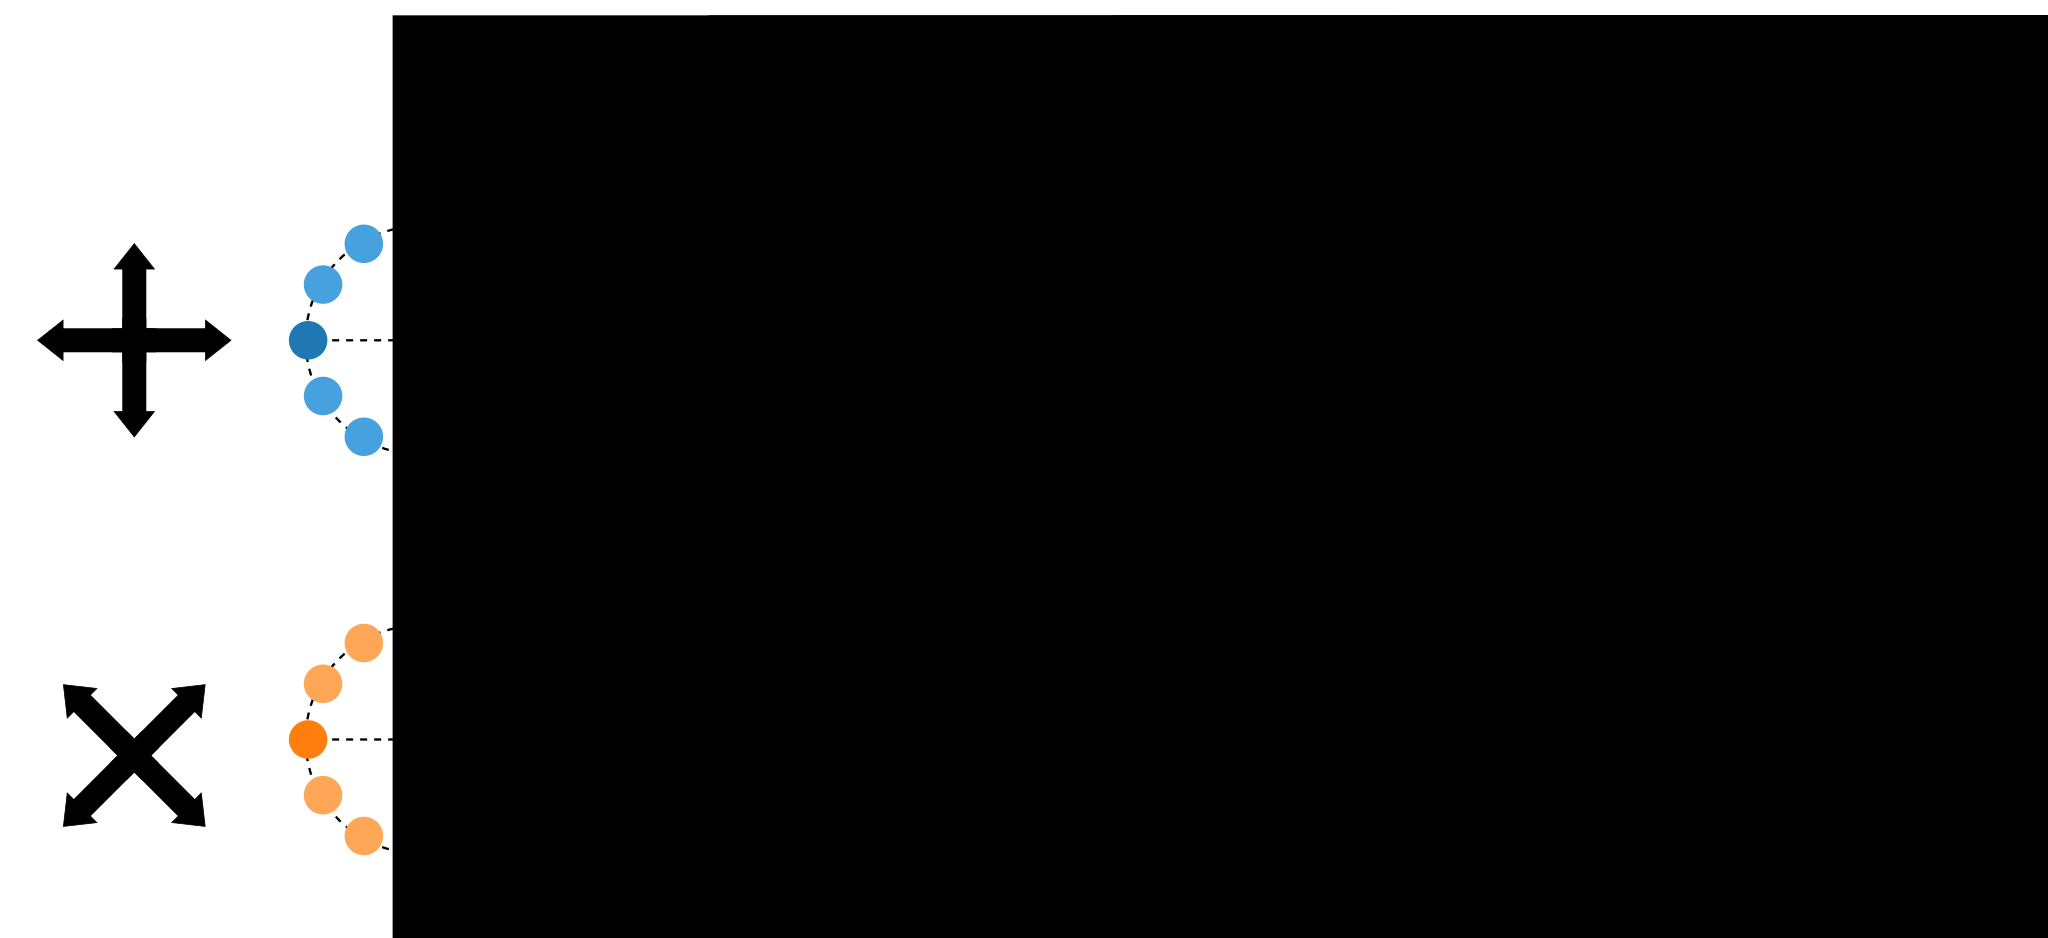
\includegraphics[width=0.8\linewidth]{images/waveimg2.pdf}
    \end{center}
    \caption[Gravitational wave polarisations]{
        Consider a 2-dimensional ring of free-floating particles in the $x$-$y$-plane. A gravitational wave that passes through the ring in the $z$-direction (out of the page) will alternately stretch and compress the ring in two orthogonal axes out of phase. The upper image shows the effect of a plus-polarised wave, the lower image shows the effect of a cross-polarised wave.
        }\label{fig:wave}
\end{figure}

\end{colsection}

% ~~~~~~~~~~~~~~~~~~~~

\subsection{Detecting gravitational waves}
\label{sec:gw_detecting}
\begin{colsection}

\begin{figure}[p]
    \begin{center}
        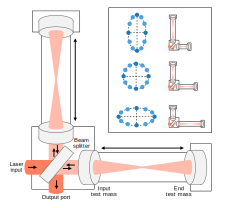
\includegraphics[width=0.75\linewidth]{images/detector.pdf}
    \end{center}
    \caption[A Michelson interferometer used as a gravitational wave detector]{
        A Michelson interferometer used as a gravitational wave detector. As a wave passes through the relative lengths of the arms will change, as shown (highly exaggerated) in the inset. This will reduce or increase the distance the laser light travels through each arm and therefore alter the output interference signal. Adapted from \citet{GW150914_detectors}.
        }\label{fig:detector}
\end{figure}

As described above, gravitational waves manifest as alternately stretching and compressing spacetime along perpendicular axes. The method used for detecting these waves requires observing how two test masses move relative to each other as the wave passes through. This is done using a Michelson interferometer with two long perpendicular arms \citep{BIGbirmingham}, as shown in \aref{fig:detector}. The input laser is split into two by a beam spitter and each beam is sent into one of the arms, where they are reflected multiple times between two mirrored test masses. When they exit the arms the beams are recombined to form a single output. Should the distance either beam travels change relative to the other the change in the resulting interference pattern will be detected. The test masses are suspended by a complex vibration isolation system in order to reduce any outside interference, such as from man-made vibrations or seismic events.

\begin{figure}[t]
    \begin{center}
        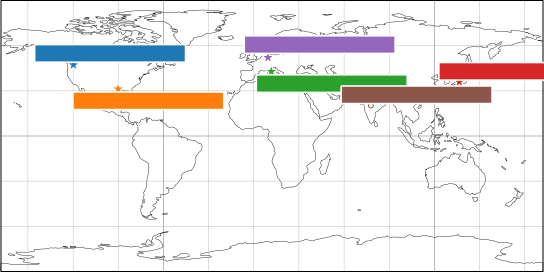
\includegraphics[width=0.95\linewidth]{images/global.pdf}
    \end{center}
    \caption[Locations of gravitational wave detectors]{
        Locations of current and proposed gravitational wave detectors around the globe.
        }\label{fig:global}
\end{figure}

Several of these detectors have been built around the world, to give redundancy and improve the localisation of each source. There are currently three active second-generation detectors: two \glsfirst{ligo} detectors at Hanford and Livingston in the United States \citep{LIGO}, and the \glsfirst{ego} Virgo detector in Italy \citep{Virgo}. In addition the older GEO600 detector in Germany is still used primarily as a test system \citep{GEO600}, the Japanese \glsfirst{kagra} is under construction \citep{KAGRA} and in the next decade work should begin on LIGO-India \citep{LIGO_India}. The three current detectors form a global network as the \glsfirst{lvc}, with KAGRA expected to join before the end of 2019 \citep{LIGO-Virgo, LIGO-Virgo-KAGRA}.

In the longer term the third generation of larger and more sensitive gravitational wave telescopes is already being planned, including the Einstein Telescope \citep{EinsteinTelescope} and the Cosmic Explorer \citep{CosmicExplorer}. As well space-based detectors are being built, such as the \glsfirst{lisa} \citep{LISA}, which would be free from the seismic noise limit and therefore could detect lower-frequency gravitational waves.

\end{colsection}

% ~~~~~~~~~~~~~~~~~~~~

\subsection{Sources of gravitational waves}
\label{sec:gw_sources}
\begin{colsection}

Any accelerating mass will generate gravitational waves as it moves through spacetime, as long as the motion is not spherically symmetric (e.g.\ a rotating disk or a uniformly expanding sphere) \citep{BIGcardiff,BIGparis}. In practice it is impossible to detect gravitational waves from anything but the most massive cosmological objects moving at the fastest speeds, as only they will produce strains that are at all detectable.

A continuous source of gravitational waves will be generated by two massive objects orbiting one another \citep{GW_sources}, and the loss of energy from the system in the form of gravitational waves will slowly cause the orbiting distance of the two objects to shrink. The first binary pulsar was discovered in 1974 \citep{HulseTaylor}, and after repeated observations it was apparent that the orbital period of the two stars was decreasing in perfect alignment with the predictions given by general relativity. This was the first real evidence, albeit indirect, of the existence of gravitational waves, and the discovery of the Hulse-Taylor pulsar was deemed so significant that its discoverers were awarded the Nobel Prize in 1993 \citep{HulseTaylor2}.

Due to the loss of energy in the form of gravitational radiation any binary orbit will eventually decay enough that the two objects collide. As the orbital distance decreases so will the period, resulting in the objects rotating faster and the system emitting gravitational waves at a higher frequencies. This will produce a characteristic `chirp' signal until the two objects merge and produce a huge burst of energy \citep{GW_sources, BIGparis}. The more massive the objects in the system the stronger the signal produced, and so the ideal binary systems for gravitational wave detections are binary neutron stars (BNS), binary black holes (BBH) or neutron star-black hole (NSBH) binaries. The first direct detection of gravitational waves, GW150914, was produced by a binary black hole system \citep{GW150914}. The `chirp' signals recorded in the LIGO detectors on the 14th of September 2015 are shown in \aref{fig:chirp}. Note the fractional strain on the $y$-axis is of the order of $10^{-21}$, meaning the \SI{4}{\kilo\metre}-long LIGO detector arms changed in length by a fraction of the size of a proton.

\begin{figure}[t]
    \begin{center}
        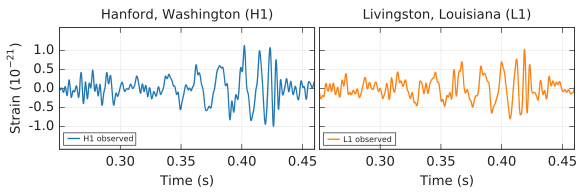
\includegraphics[width=\linewidth]{images/chirp.pdf}
    \end{center}
    \caption[The first detection of gravitational waves]{
        The first detection of gravitational waves, recorded in the LIGO Hanford detector (on the left) and then approximately \SI{7}{\milli\second} later in the LIGO Livingston detector (on the right). The expected `chirp' signal characteristic of a binary coalescence is visible --- a wave of increasing frequency that reaches a maximum and then collapses. Adapted from \citet{GW150914}.
        }\label{fig:chirp}
\end{figure}

The LIGO detectors became operational in 2002 and observed on-and-off until 2010 without detecting any gravitational wave signals, when they were taken offline in order to upgrade into Advanced LIGO \citep{LIGO_initial, LIGO_advanced}. The detectors were recommissioned in 2015, and almost immediately detected the first signal, GW150914, as mentioned above \citep{GW150914}. The first LIGO observing run (O1) \glsadd{o1} lasted from September 2015 to January 2016, and during that time two additional signals were detected \citep{LIGO_O1}. All three detections were identified as being produced by coalescing black hole binaries, and although at the time one (LVT151012) was below the $5\sigma$ significance level it has since been upgraded to a significant detection and reclassified as GW151012 \citep{GW_catalog}.

\newpage

The second observing run (O2) \glsadd{o2} took place from November 2016 to August 2017. This run saw the first observation of gravitational waves from a binary neutron star, GW170817 \citep{GW170817}, as well as the addition of the Virgo detector to the network. In total eleven gravitational wave events were detected during O1 and O2, ten from binary black holes and just the one (GW170817) from a binary neutron star \citep{GW_catalog}.

After a few short engineering runs the third observing run (O3) \glsadd{o3} begun on 1 April 2019. At the time of writing it is currently ongoing, and after a short break during October is expected to run until May 2020. This is the first run to include three detectors from the beginning, and KAGRA is expected to join before the end of 2019. This run also marked the start of public alert releases; during O1 and O2 alerts were only released to groups who had signed memoranda of understanding with the LVC (the GOTO Collaboration was one of these groups). In the first 5 months of O3, from the start of April to the end of August 2019, the LVC released 32 alerts\footnote{Public alerts are available at \url{https://gracedb.ligo.org/superevents/public/O3/}}. Of these 7 were ultimately retracted as false alarms, leaving 25 due to real astronomical signals.

As O3 is currently ongoing the LVC has not yet published final values or mass estimates for any of these events. As such they are still treated as candidates, with provisional signal designations and preliminary classification probabilities. Of the 25 non-retracted events 20 are currently classified as originating from binary black hole systems ($P_\text{BBH}>90\%$). Only one is likely from a binary neutron star (S190425z), one is classed as a likely neutron star-black hole binary (S190814bv), and one (S190426c) has an uncertain classification: a 49\% probability as coming from a binary neutron star, 24\% coming from a `MassGap' object (a theorised object with a mass between a neutron star and a black hole) and 13\% from a neutron star-black hole binary (the remaining 14\% is the chance the signal is from a non-astrophysical source, i.e.\ detector noise). The remaining two events both have over 50\% non-astrophysical probability but have not been formally retracted by the LVC.\@

\end{colsection}

% ~~~~~~~~~~~~~~~~~~~~
\newpage
\subsection{On-sky localisation}
\label{sec:gw_localisation}
\begin{colsection}

One problem with the interferometer detectors is that alone they are very poor at localising the direction a signal originates from. It is possible to estimate a rough direction from polarisation of the signal, and the distance to the origin can be estimated from the signal strength, however multiple detectors are really needed to get more accurate sky localisations \citep{GW_localisation, GW_localisation2}. With two detectors the difference between the arrival time of a signal at each allows the direction to the source to be narrowed down, based on the distance between the two detectors and knowing that gravitational waves propagate at the speed of light. However this will only be able to locate the source to a annulus on the celestial sphere perpendicular to the line between the detectors, and as shown in \aref{fig:triangulate} at least three detectors are needed to triangulate the source location. The skymaps for GW170817, shown in \aref{fig:170817_skymaps}, show how the contribution from multiple detectors drastically reduced the on-sky area. Even with the three current detectors sources can typically only be localised to areas of tens to hundreds of square degrees at best, and only if the signal is detected in all three.

\begin{figure}[t]
    \begin{center}
        \includegraphics[width=0.45\linewidth]{images/triangulate_1.pdf}
        \includegraphics[width=0.45\linewidth]{images/triangulate_2.pdf}
    \end{center}
    \caption[Localising signals using gravitational wave detectors]{
        Localising signals using gravitational wave detectors. With just two detectors sources can only be localised to a ring on the sky (shown on the left, for three different sources). The addition of a third detector means sources can be triangulated to where the rings intercept (shown on the right).
        }\label{fig:triangulate}
\end{figure}

\begin{figure}[p]
    \begin{center}
        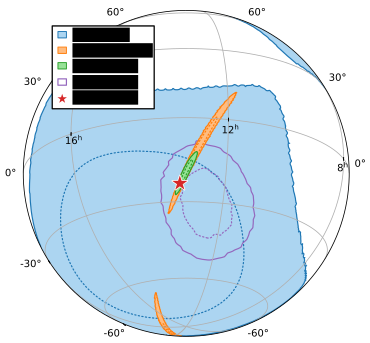
\includegraphics[width=\linewidth]{images/skymaps.pdf}
    \end{center}
    \caption[Skymaps for GW170817]{
        Skymaps for GW170817, produced from the single Hanford detector (in \textcolorbf{NavyBlue}{blue}), both Hanford and Livingston (\textcolorbf{Orange}{orange}) and all three detectors (\textcolorbf{Green}{green}). The final \textit{Fermi} GBM skymap is also shown in \textcolorbf{Purple}{purple}, and the location of the counterpart source is marked by a \textcolorbf{Red}{red} star. Solid lines show 50\% confidence regions, dashed lines 90\% regions.
        }\label{fig:170817_skymaps}
\end{figure}

\end{colsection}

% ~~~~~~~~~~~~~~~~~~~~

\end{colsection}

% ########################################

\newpage
\section{Multi-Messenger Astronomy}
\label{sec:multi}
\begin{colsection}

% ~~~~~~~~~~~~~~~~~~~~

\begin{colsection}

\todo{this is worded weirdly}
\todo{more sources?}



Binary mergers involving neutrons stars are suggested as possible sources of short duration gamma ray bursts (SGRBs) \citep{GW-NSbinaries}. They would also potentially produce kilonovae, from which it might be possible to detect other forms of electromagnetic signal. On the other hand BBH mergers are thought to be unlikely to produce EM emission, as the stellar-mass black holes would not be surrounded by much orbiting matter with which to interact \citep{GW-BHbinaries,GW150914followup}.

As opposed to the continuous sinusoidal waves produced by massive binaries, any particularly cataclysmic astronomical event is thought to produce a burst of gravitational waves. Compact binary mergers are one source of these bursts, but more sudden ones are thought to include be produced in core-collapse supernovae \citep{GW-supernovae}. Unlike binary systems the exact form of GW burst waveforms are unknown. As such gravitational wave detectors are likely to detect new and unexpected sources.

The term \emph{multi-messenger} astronomy is often used to describe the search for GW candidates. It emphasises the fact that the hunt is focused on multiple `types' of observation in addition to gravitational wave detections --- across the EM spectrum as well as neutrino detections. The observation of EM counterparts of transient GW sources would provide several scientific benefits \citep{LIGO-EM, LIGO-firstrun-2012}. Most obviously, an EM detection would help massively in the localisation of the source, potentially the identification of a host galaxy and measurement of a redshift. An associated EM observation would also assist with identification of the nature of the source. While a gravitational wave is generated by the motion of the source in spacetime, any EM signal would be produced either from direct outflows or interactions of the matter with the surrounding medium. In the longer term these observations should be useful in determining cosmological parameters such as $H_0$.

\end{colsection}

% ~~~~~~~~~~~~~~~~~~~~

\subsection{The advantage of multi-messenger observations}
\label{sec:mma_advantages}
\begin{colsection}

\todo{do it}

\end{colsection}

% ~~~~~~~~~~~~~~~~~~~~

\subsection{Finding optical counterparts to gravitational wave detections}
\label{sec:followup}
\begin{colsection}

As the sky map is so large, particularly in the early years of GW detections, the options are either to try and cover as much of the area as possible by using wide field-of-view telescopes or to selectively focus on regions of the sky where the candidate is most likely located.

The `galaxy strategy' optimises the follow-up observations by focusing on any galaxies within the provided sky map \citep{LIGO-galaxys}. Notably this was used by the \emph{Swift} satellite as its X-ray and UV instruments have particularly small fields of view \cite{LIGO-firstrun-Swift,GW150914followup-Swift}. The most important resource for such a strategy is a complete galaxy catalogue, and this will become more of an issue as the sensitivity and therefore range of the advanced detectors increases. The Gravitational Wave Galaxy Catalogue (GWGC) provided a list of galaxies within 100 Mpc \citep{LIGO-GWGC} which has been used in the first follow-up campaigns \citep{LIGO-firstrun-Swift,GW150914followup-Swift}. More work is being done as the catalogues become less complete as the detection range grows higher \citep{LIGO-galaxys,LIGO-galaxys2}.

Even with high field-of-view instruments, there is a great deal of strategy needed for observation prioritising. In most cases the sky is split into multiple fixed `tiles' for optimising observations and comparison to archival images. A GW sky map will cover a certain number of these tiles, and the selection algorithm will need to decide the order to to observe them in \citep{LIGO-tiles-dutch, LIGO-tiles-india}. At its simplest this will rank the tiles by the highest sky map probability contained within. However other considerations include the optimum time for observing based on airmass, the setting time of each tile, the location of the sun and moon, slew time between each observation and so on.

Whenever a gravitational wave is detected a sky map will be sent out to multiple facilities across the Earth (and above it). Therefore it is also important to consider optimisation of the overall EM search effort between multiple institutions \citep{LIGO-optimal,LIGO-optimal2}. Individual groups of institutions in Italy \citep{LIGO-italy} and Australia \citep{LIGO-aus} have already considered such collaborations. \todo{ENGRAVE}

\end{colsection}

% ~~~~~~~~~~~~~~~~~~~~

\subsection{Case study: GW170817}
\label{sec:gw170817}
\begin{colsection}

\todo{do it}

\end{colsection}

% ~~~~~~~~~~~~~~~~~~~~

\end{colsection}

% ########################################

\newpage
\section{The Gravitational-wave Optical Transient Observer}
\label{sec:goto}
\begin{colsection}

% ~~~~~~~~~~~~~~~~~~~~

\begin{colsection}

The \gls{goto}\footnote{\url{https://goto-observatory.org/}} is a project dedicated to detecting future optical counterparts of gravitational wave sources by employing a wide-field approach to be able to localize such counterparts early. The first prototype instrument was inaugurated at the Roque de los Muchachos Observatory on La Palma, Canary Islands in July 2017 and is shown in \aref{fig:goto_photo}. \gls{goto} uses arrays of \SI{40}{\cm} \glspl{ut} on a single fast-slewing mount. This modular approach allows the project to scale to large fields of view in a cost-effective manner. A full instrument will have 8 of these \glspl{ut} per mount, giving an overall field of view of \SI{40}{\square\deg} with a pixel scale of \SI[per-mode=symbol]{1.2}{\arcsec\per\pixel} and a limiting magnitude of \about20 in each two minute exposure. Each UT has a set of wide white and coloured filters to assist source characterisation.  An additional instrument with 8 more \glspl{ut} on a second mount is planned to be co-located in a second dome on La Palma, which will double the instantaneous field of view to \SI{80}{\square\deg}, allow the sky to be surveyed at a higher cadence and give more options for transient follow-up. A southern node is also planned for Australia.

\begin{figure}[t]
    \begin{center}
        \includegraphics[width=11cm]{images/goto_photo.jpg}
    \end{center}
    \caption[The GOTO prototype instrument]{
        The GOTO prototype instrument on La Palma, with four of the eventual eight unit telescopes.
    }\label{fig:goto_photo}
\end{figure}

\gls{goto} is designed as a robotic, wide-field transient detection telescope. Under normal circumstances the telescope will carry out an all-sky survey, based on a fixed grid of tiles. Each tile corresponds to the \SI{40}{\square\deg} field of view of the 8 \glspl{ut} observing neighbouring patches of sky, as shown in \aref{fig:tiles}. The all-sky survey will aim to obtain a high-cadence at an appropriate depth, mapping the entire visible sky several times a week. The high cadence will ensure that there are very recent reference images available to allow detection of objects using difference imaging.

\begin{figure}[t]
    \begin{center}
        \includegraphics[width=11cm]{images/tiles.pdf}
    \end{center}
    \caption[M31]{
        A single commissioning image of M31, showing the wide field of view of each unit telescope. The full 8 unit telescope array will cover an area of approximately 40 square degrees, which forms a single survey tile.
    }\label{fig:tiles}
\end{figure}

\end{colsection}

% ~~~~~~~~~~~~~~~~~~~~

\subsection{Hardware design}
\label{sec:goto_design}
\begin{colsection}

\todo{WIP}
\todo{Include lots of pictures, labeled diagram of bits}

\end{colsection}

% ~~~~~~~~~~~~~~~~~~~~

\newpage
\subsection{Deployment plan}
\label{sec:goto_expansion}
\begin{colsection}

\todo{WIP}

Starting with 4 in the North, 1 mount.

Then 8 on the 1 mount, soon (TM).

Then another 8.

Then Australia, hopefully.

\newpage

\begin{figure}[p]
    \begin{center}
        \includegraphics[width=\linewidth]{images/orm_labelled.png}
    \end{center}
    \caption[Locations of major telescopes on La Palma]{
        Locations of major telescopes at the ORM on La Palma. GOTO, marked in \textcolorbf{BlueGreen}{blue}, is located on the east side of the observatory, close to the edge of the Caldera.
    }\label{fig:orm}
\end{figure}

\begin{figure}[p]
    \begin{center}
        \includegraphics[width=\linewidth]{images/orm_east_labelled.png}
    \end{center}
    \caption[The location of GOTO on La Palma]{
        The location of GOTO on the eastern edge of the ORM on La Palma, marked in \textcolorbf{BlueGreen}{blue}. The surrounding telescopes are also labelled, including the other Warwick-operated telescopes (W1m and SuperWASP) in \textcolorbf{Orange}{orange} and the Sheffield-Durham operated pt5m (on the roof of the WHT building) in \textcolorbf{Green}{green}.
    }\label{fig:orm_east}
\end{figure}

\clearpage

\end{colsection}

% ~~~~~~~~~~~~~~~~~~~~

\end{colsection}

% ########################################

\newpage
\section{Thesis outline}
\label{sec:outline}
\begin{colsection}

\todo{This is my thesis!} This thesis is about GOTO, a telescope with the primary mission to detect counterparts to gravitational wave sources.
%
\begin{itemize}
    \item In \nref{chap:hardware} I blah.
    \item In \nref{chap:gtecs} I blah.
    \item In \nref{chap:autonomous} I blah.
    \item In \nref{chap:scheduling} I blah.
    \item In \nref{chap:tiling} I blah.
    \item In \nref{chap:alerts} I blah.
    \item In \nref{chap:commissioning} I blah.
    \item In \nref{chap:multiscope} I blah.
    \item In \nref{chap:conclusion} I blah.
\end{itemize}
%
Let's begin \ldots

\end{colsection}

% ########################################
